\section{IoTサービスの構造と事例}
IoTサービスとは、IoT機器とサーバが連携し利便性を提供するものである。

株式会社ルナネクサスでは、太陽光発電事業を展開している事業主に対し、発電に係る機器の状態や、発電量等を可視化できるサービスを展開している。
太陽光発電は、太陽光パネルと発電した電力を送電する為の「パワーコンディショナ」と呼ばれる機器で成り立っている。
株式会社ルナネクサスでは、そのパワーコンディショナに独自に開発したIoT機器を取り付け、発電量や発電機器の異常などを収集する。
収集したデータは、SORACOM Airという携帯電話網を利用したインターネット接続サービスを使用してインターネット上にあるサーバへ送信される。
サーバ上では、各IoT機器から送られてきた情報を蓄積し、可視化する。
これによって、発電事業を展開している事業主に、各発電所まで行かなくても発電量や発電機器の異常等を確認することができる、という利便性を提供している。
SORACOM Airとは、後術するIoT機器向けのインターネット接続サービスの事である。
図\ref{fig:lunafig}は株式会社ルナネクサスのIoTサービスイメージである。
\begin{figure}[htbp]
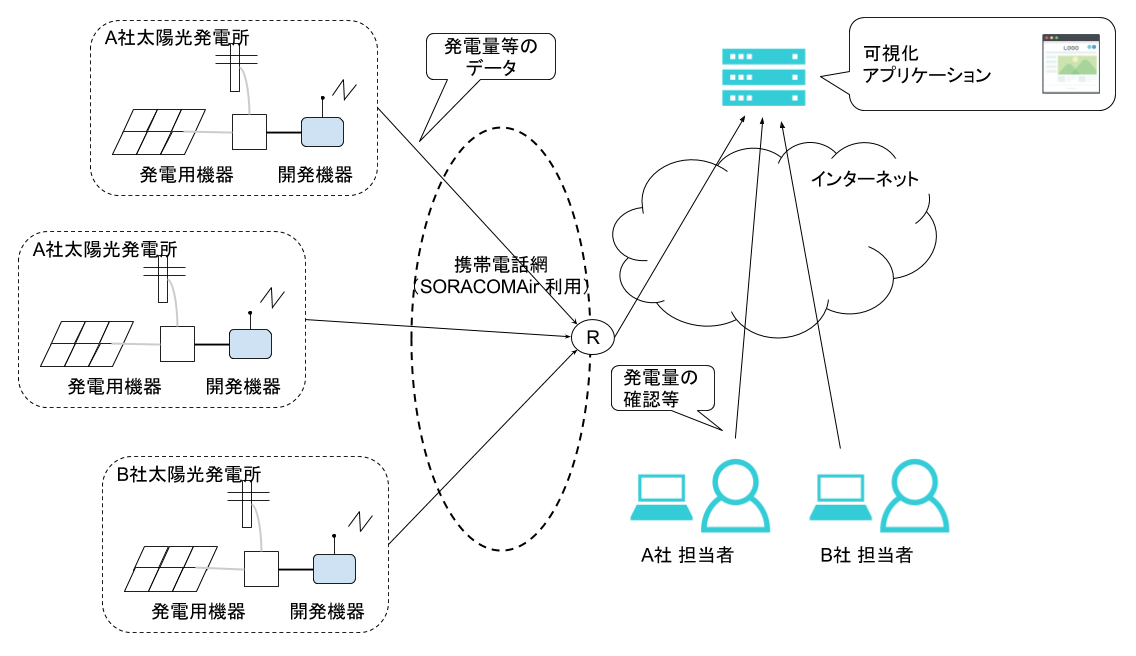
\includegraphics[width=16cm]{images/lunafig.png}
\caption{株式会社ルナネクサス サービスイメージ図}
\label{fig:lunafig}
\end{figure}
太陽光発電所は僻地にあることが多いので、利用できるネットワークが無いことが多い。
このことから、インターネットへの接続にSORACOM Airを選択した。

しかし、SORACOM Air回線は、プライベートアドレスを使用しており、IoT機器からの通信は通過するものの、インターネット側からPingなどによる確認を行うことが出来ない。
そのため、各IoT機器の監視とメンテナンスの為に、VPNを利用し、定期的にVPN越しにログインすることで監視を行っている。
VPN越しにログインするためには、各IoT機器にVPNクライアントを導入し、新たにVPNサーバをたち上げる必要があった。
また、手動で各機器へログインすることは、手間である。

\section{IoTサービスの提供者の課題}
前項で述べたとおり、株式会社ルナネクサスでは、各IoT機器のメンテナンスと状態の確認の為に、VPNを利用して遠隔から手動でログインすることを行っている。
各機器のメンテナンスは頻繁には行っていないが、各IoT機器の稼働の確認は定期的に行っている。
現在、IoT機器は十数台しかないが、今後、増えていく事が予想されるため、各IoT機器の稼働の確認が大きな負担となる。

この問題について調べる為に、株式会社ルナネクサスへインタビューを行ったところ、次のような要望があった。
\begin{itemize}
\item 単純に機器が起動し、動作している事が確認できれば良い
\item 欲を言うと、CPUの温度等も確認できれば良い
\item 各機器に対するVPNや監視の為の設定も簡略化できたら尚良い
\end{itemize}

\section{考察}

\subsection{岡本商店街での事例}
この問題は、岡本商店街で行った実験の際も問題となった。
岡本商店街とは、神戸市東灘区にある阪急岡本駅とJR摂津本山駅の間にある商店街のことで、
商店街の方に人流を可視化するIoTサービスを提供し商店街の活性化に役立てるといった趣旨で、2016年2月7日から2016年3月14日まで観測を行った。
人流観測とは、各地点から各地点迄をある時に移動した人数を観測するものである。
今回は、ある地点を通過した人物が以前どの地点を通過していたのかを観測したかった為、携帯電話についているWifi機能が送出する電波を利用して観測を行うこととした。
観測・分析・可視化を行うシステムの構成としては図\ref{fig:okamoto_diag1}の様になる。
\begin{figure}[htbp]
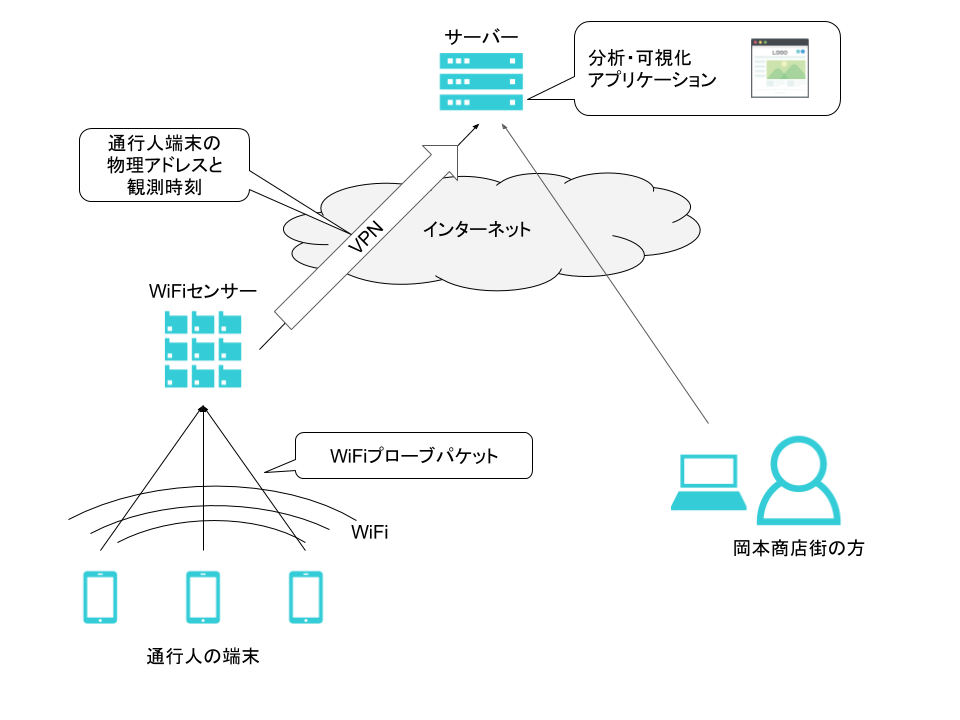
\includegraphics[width=16cm]{images/okamoto_diag1.png}
\caption{岡本商店街人流観測 構成図}
\label{fig:okamoto_diag1}
\end{figure}
各店舗に設置させてもらった観測機器は、店舗に敷設されたネットワーク回線を通して、インターネットへと繋がっている。
各観測機器は、観測したデータをインターネット上のサーバへと送信し、そのサーバの上で蓄積・分析・可視化を行う形となっている。

実験の際に、次の様な問題や負担があった。
\begin{itemize}
\item 電源が抜けている・ネットワークが切断されているといった要因で、観測できていないことがあった。
\item 上記要因にて観測できていない事に気づくことが遅れた。
\end{itemize}
これらから、IoT機器の監視が必要と考え、VPN越しにログインすることで、確認を行うこととした。
しかし、各観測機器にVPNを介してログインすることは手間であり、負担であった。
また、実験では観測機器の数が5台のみであったが、大規模に観測を行うことを考えた場合、手動での確認はとても大きな負担となる。
そのため、効率化を図る必要があったと感じる。

\subsection{岡本商店街での事例を踏まえた考察}
株式会社ルナネクサスにて問題となっていたIoT機器の監視が負担となっている問題は、岡本商店街にて行った人流観測実験でも問題となっていたため、共感する部分が多かった。
また、構成として似たような構成をとっていることから、IoT機器の監視が負担である問題を取り上げることとした。






%IoTサービスの構造の維持が必要で、維持の為に、監視が必要となっている
%また、その監視は注ぎのヨ兼を満たしている必要がある。
\begin{comment}
この考察の中で、「開発者」の視点を入れて説明してください。
誰がどのように困っているのかをはっきり説明して、そのうえでどうあるべきかの要件の説明です。
「運用者」の視点も混ざると大変だと思うので、ひとまず「開発者」=「運用者」というつもりで書いてくれていいです。
IoTサービスの開発運用の困難ということで。

このように、開発者・運用者は、構造の複雑さ・利便性から困っている。
ここから、私は、次のような点を問題として取り上げた。
\begin{itemize}
\item IoT機器の監視は必要だが、技術的な問題により、既存の監視手法では監視しづらい
%\\	株式会社ルナネクサスの事例でも、岡本商店街の事例でも、IoT機器が接続されるネットワークが様々である(になる予定である)ことから、監視が難しくなっている。
\item IoT機器の監視問題の解決の為に、開発者の負担が大きくなっている
%\\	2事例にて、機器の監視の解決の為に、開発者の負担が大きくなっていることが分かった。
\end{itemize}

これらから、IoT機器の監視に特化した機器の監視システムが必要であると感じた。
これら実験やヒアリングの結果から、監視には次のような物が求められていることが分かった。
\begin{itemize}
\item IoT機器の接続されるネットワークが、プライベートアドレスを使用していても、監視可能であること\\
	IoT機器が接続されるネットワークを予め予測することは難しい。
	そのため、IoT機器にプライベートアドレスが割り振られる可能性がある。
	そのような状況でも監視することができる必要がある。
\item ネットワークが違っていても、一つの画面で確認できること\\
\item IoTサービスの変更が不要であること\\
	サーバの変更は開発者への負担となるため、サーバの変更を避けたい。
\item 監視サーバを立てる必要がないこと\\
	新たに監視サーバを立てることは、設定や構築作業が必要となるため、開発者の負担となる。
	そのため、新規に監視サーバを立てる必要が無いことが求められる。
\end{itemize}
\end{comment}

